\documentclass[a4paper,12pt]{article}

\usepackage{../my_pkg}


\title{Project 2: Drawing Basic Charts in Processing\\
\vspace{5pt}\normalsize (Adapted from an assignment created by Carlos Scheidegger)}
\SetDocumentFooter{}{}

\begin{document}

\maketitle

\section{Objectives}

\myparagraph{In this assignment you will learn the basics of Processing, and create a few Processing sketches that implement basic visualizations. These will be building blocks for future assignments, so take care to use good software engineering practices. You will create 3 sketches.}

\section{Ground Rules}

\groundrules

\section{Getting Started}


\myparagraph{We will be using a git repository for submissions throughout the semester. A script will automatically scrape your solution at the deadline. \textbf{Please follow these instructions carefully.} If done incorrectly, we won't get your submission, and you will get a 0.}


\begin{itemize}
\item \textbf{Install git} on your local machine. 
\begin{itemize}
\item For Windows, I recommend TortoiseGit (\url{https://tortoisegit.org/}). You will also need the Git for Windows tools (\url{https://git-scm.com/download/win}).
\item For Mac, install xcode (\url{https://developer.apple.com/xcode/}) and then the command-line tools (\url{http://railsapps.github.io/xcode-command-line-tools.html}). 
\item For Linux, git should already be installed. If not, use the appropriate package manager (e.g.\ apt or yum) to install it.
\end{itemize}

\item \textbf{Create Account:} Create a GitHub account, if you don't already have one (\url{https://github.com/}). A GitHub Education account is optional (\url{https://education.github.com/discount_requests/new}).

\item \textbf{Setup Repository:} Visit (\url{https://classroom.github.com/a/0JcYQJsF}) to setup your repository with the skeleton code already added. It is important that you use this url. It attached your repository to our class.


\item \textbf{Clone the repository:} Once the repository is created (this can take a few minutes) determine the remote path and pick a local directory for code. Clone the project locally (i.e.\ \textit{git clone $<$url\_to\_repository$>$ $<$path\_to\_local\_directory$>$}).

\item \textbf{Edit your code:} Use existing \textbf{project2} directory for storing/editing your code. If you put it anywhere else, our scripts will fail (and so will you). As you work, make sure you add the files to the repository (i.e.\ \textit{git add}), commit the changes (i.e.\ \textit{git commit}), and push changes to the remote server (i.e.\ \textit{git push}). \underline{Be sure to frequently commit and push your work!}

\item \textbf{Submission:} We will pull from the last commit before the deadline. Make sure to push your code one last time before you're done. If you fail to do this, we won't get your files.  

\item \textbf{Verify:} You can verify that your files have been properly uploaded by checking the Code page on the GitHub website.

\end{itemize}



\section{Assignment Instructions}

\begin{itemize}

\item Download and familiarize yourself with Processing (\url{http://processing.org/download/}). Use the available tutorials (\url{http://processing.org/tutorials/}) and examples (\url{http://processing.org/examples/}) to help you understand how Processing works.

\item Create a data file. Your data file should be a csv format file (\url{http://www.computerhope.com/issues/ch001356.htm}). The file should contain the following headers \{YEAR, VALUE0, VALUE1, PARTY\} and values $\Big[$\{1992, 7.30, 88, DEM\}, \{1996, 5.60, 43, DEM\}, \{2000, 4.00, 76, REP\}, \{2004, 5.70, 90, REP\}, \{2008, 5.00, 12, DEM\}, \{2012, 8.30, 14, DEM\}, \{2016, 4.90, 50, REP\}$\Big]$.

\item Create a sketch with 600x600 resolution that opens a file dialog box (\url{http://processing.org/reference/selectInput_.html}) and loads a selected csv data file. You can start with the skeleton code provided on Canvas.

\item With the given data file, draw a BAR CHART for the data (you get to pick which variables to use).


\begin{center}
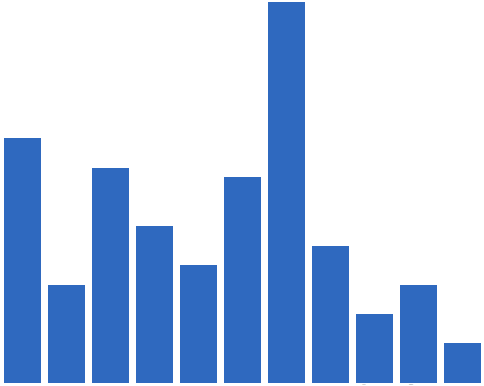
\includegraphics[width=4cm, height=3cm]{../images/barchart.png}
\end{center}

\item Create a 2nd sketch (same resolution and dialog box), and draw a LINE CHART for the data (again you get to pick which variables to use).


\begin{center}
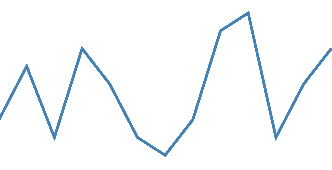
\includegraphics[width=4cm]{../images/linechart.png}
\end{center}


%\item Create a 3rd sketch (same resolution and dialog box), and draw a LINE CHART on top of a BAR CHART with the data.

%\begin{center}
%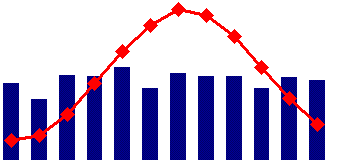
\includegraphics[width=4cm]{../images/bar_and_line_chart.png}
%\end{center}



\item Modify your sketches such that they use additional visual channels to encode additional variables. Consider using color, size, shape, depth, etc. Your selection and their implementation will have an impact on your grade.

\item Add embellishments of your choice. These can include but are not limited to: axis lines, labels, and tick marks. Consider the margins for your embellishments (try to pick good values for the tick marks and a good number of them---not too many and not too few). Your selection and their implementation will have an impact on your grade.

\item Make your visualizations robust by designing them to support any data (number of elements or value range) and by designing them to support any size or aspect ratio of canvas. You will reuse this code in future assignments, so functionalities will be particularly important.

\end{itemize}


\section{Submission}

\submission{project2}



\section{Grading and Feedback}

\feedback{
\begin{itemize}
	\item 2 Visualizations - 6 points (basic implementation 3 points each)
	\item Additional Visual Channels - 1.5 points 
		\begin{itemize}
    		\item 0.5 points for none used
    		\item 1.0 point for a few
            \item 1.5 points for many
		\end{itemize}
	\item Embellishment - 1.5 points 
		\begin{itemize}
    		\item 0.5 points for none used
    		\item 1.0 point for some
            \item 1.5 points for a lot
		\end{itemize}
	\item Code Professionalism - 1 points
		\begin{itemize}
            \item 0.5 no comments, no classes, "hard coded" values
            \item 0.75 minimally commented, few "hard coded" values
            \item 1.0 commented, properly used classes, few "hard coded" values
		\end{itemize}
\end{itemize}
}




\newpage


\begin{center}
{\huge Project 2 Peer Review}
\end{center}




\StartTable{Visual Design}

\AddMultipleChoiceElement{Visual Channels}
	{What visual channels were used to encode data? }
    { 
     \AddMCColumn{1.65cm}{\choice Position	\\ \choice Depth	\\ \choice Angle}
     \AddMCColumn{1.95cm}{\choice Curvature	\\ \choice Shape	\\ \choice Length}
     \AddMCColumn{2.3cm}{\choice Area		\\ \choice Volume  	\\ \choice Luminance/\\\ \ Saturation}
     \AddMCColumn{1.95cm}{\choice Color Hue	\\ \choice Texture	\\ \choice Motion/\\\ \ Animation}
    }
        
\AddElement{Intended/Unintended Encodings}
	{Do all of the visual encoding appear to be intended, or were some accidentally created?}
        {\choice Many\\Unintended}
        {\choice Few\\Unintended}
        {\choice All\\Intended} 
        
\AddElementExtended{Expressiveness of Encodings}
	{Are the visual encodings attached to the correct type of data for that 
    	encoding (i.e.\ are quantitative data attached to quantitative 
        encodings and categorical data to categorical encodings)?}
    {\choice Many\\Errors}
    {\choice Few\\Errors}
    {\choice Correctly\\Assigned} 
            
\AddElement{Effectiveness of Encodings}
	{Have the maximally effective visual encodings been selected in all cases? }
    {\choice Many\\Ineffective}
    {\choice Few\\Ineffective}
    {\choice Most\\Effective} 
        
\AddElement{Effective Use of Color}
	{Is color used in a same fashion? Do the colors chosen and the application 
    	of those colors make the visualization effective?}
    {\choice Mostly\\Ineffective}
    {\choice None\\Used}
    {\choice Highly\\Effective} 

\EndTable  

\vspace{15pt}

\StartTable{Design Considerations}

\AddElement{Clear, Detailed, and Thorough Labeling}
   	{Is appropriate and complete labeling used throughout or do 
      	missing labels require assumptions about the data?}
    {\choice No labels}
    {\choice Some Missing labels}
    {\choice Completely labeled} 
        
\AddElement{Missing Scales}
   	{Are scales provided for the data?}
	{\choice No Scales}
	{\choice Some Missing Scales}
	{\choice All Scales Present} 

\AddElement{Missing Legend}
	{Is a legend provided for the data? Does the legend provide useful 
    	information?}
	{\choice No Legend}
	{\choice Incomplete Legend}
	{\choice Complete Legend} 
        
        
\EndTable  


\StartTable{Design Considerations (cont.)}

\AddElement{Scale Distortion}
	{Is any scale distortion or deception used in the visualization?}	
	{\choice Severe Distortion}
	{\choice Minor Distortion}
	{\choice No Distortion} 
        
\AddElement{Lie Factor}
	{Is there any lie factor? How extreme is the lie factor?}
	{\choice Major Lie}
	{\choice Minor Lie}
	{\choice No Lie} 

\AddElement{Data/Ink Ratio}
	{Is the data to ink ratio reasonable? Could it be more efficient?}
	{Way Too $\square$~Little / $\square$~Much Ink}
	{Slightly Too $\square$~Little / $\square$~Much Ink}
	{\choice Perfect Amount of Ink} 
        
\AddElement{Chart Junk, Embellishments, Aesthetics}
	{Are appropriate embellishments used? Are the embellishments 
    	distracting? Do the embellishments add to the visualization?}
	{Way Too $\square$~Few / $\square$~Many Embellishments}
	{A Bit Too $\square$~Few / $\square$~Many Embellishments}
	{\choice Perfect Number of Embellishments} 
        
\AddElement{Data Density}
	{Has too much data been included in the visualization making 
    	interpretation difficult? } 
	{\choice Too Sparse}
	{\choice Expected}
	{\choice Too Dense} 
        
\EndTable  
        




\end{document}


